\subsection{Actuator board} %Lennie
The actuator board is a board made to control the solenoids for the markers and the torpedoes. The board can have one or two inputs and four outputs. One input can power either two or four actuators depending if the two pins located below the fuses named pwr\_bridge is bridged. The power inputs can be at any level between 0V to 24V. The actuator board does not have any current regulators for the outputs, this is because each output will only be activated for a short time, when the markers get dropped or torpedoes shot. The solenoids that the outputs will power will also be submerged in water, so the heat will not be a problem. Each solenoids is controlled by a digital high/low signal that is sent from a CAN-card. The experimenal actuator board can be seen in fig. \ref{ActuatorImgText}.

\begin{figure}[!ht]
	\begin{center}
		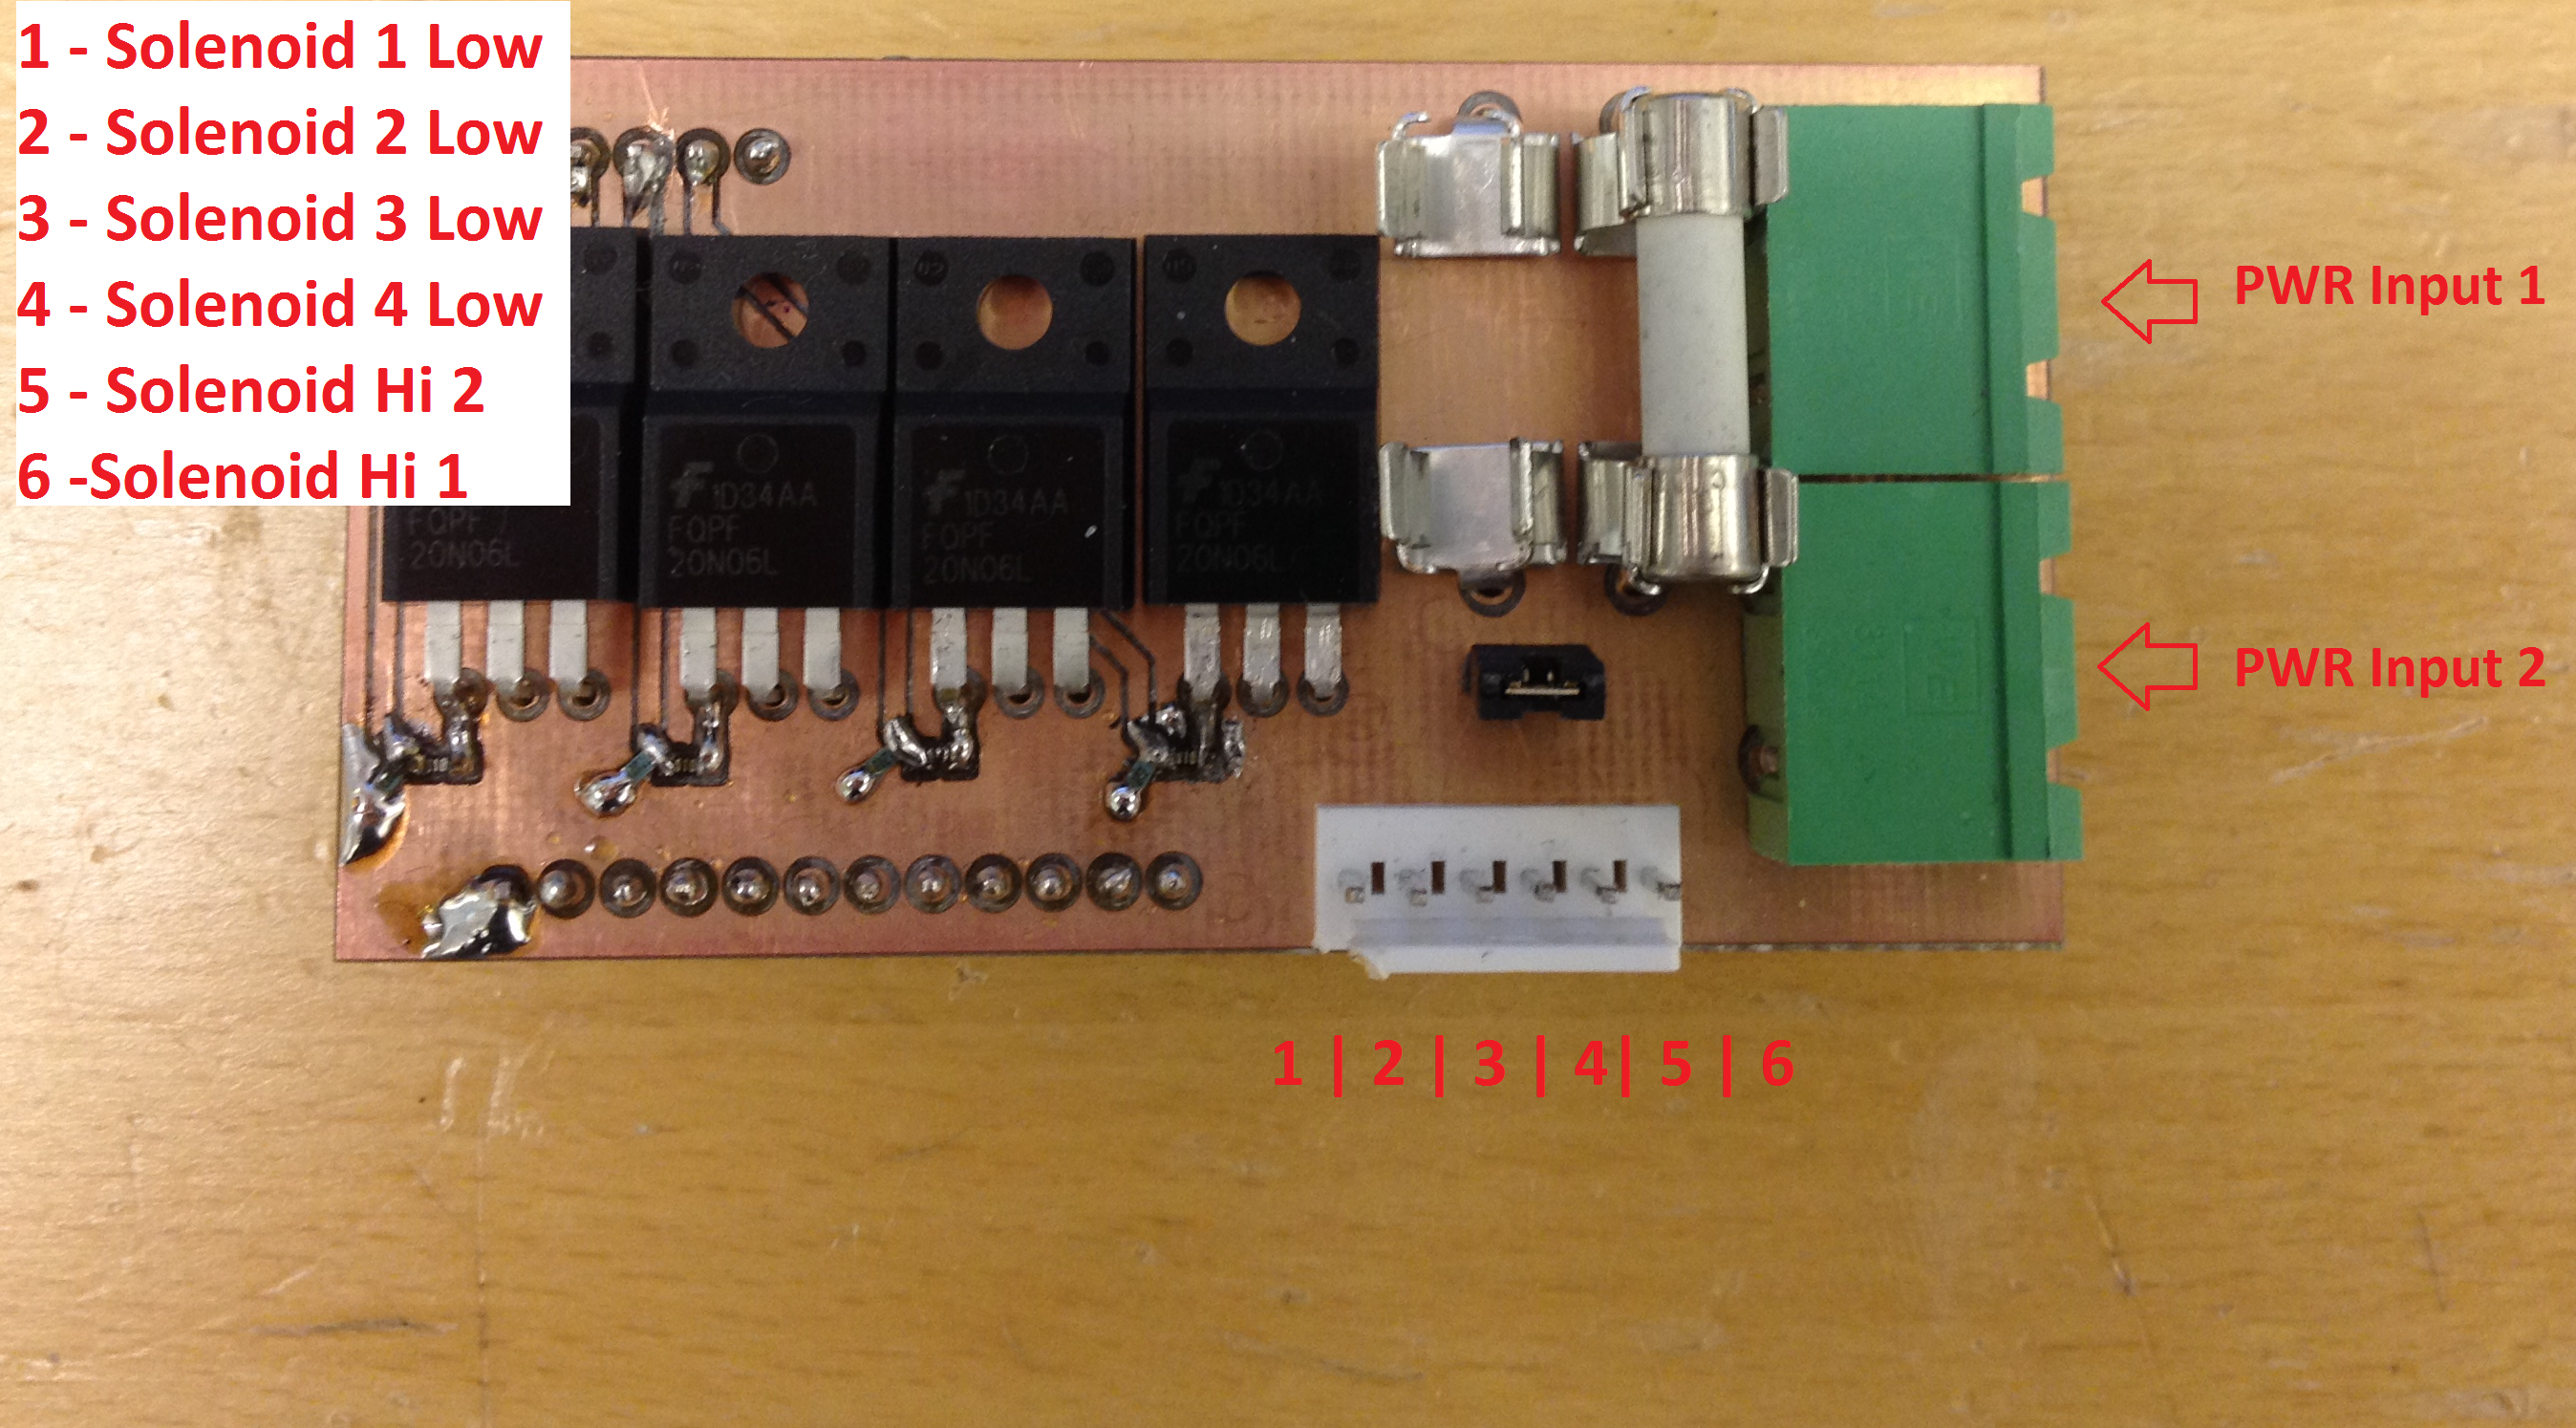
\includegraphics[width=80mm]{./Images/Electronics/ActuatorImgText.png}
		\caption{Picture of the experimental actuator board}
		\label{ActuatorImgText}
	\end{center}
\end{figure}


	
